\vspace{.08in}
\noindent \textbf{Fast ROMs for Turbulence.} (Tasks 2 and 3.)
The goal of this task is to push the state-of-the-art for ROM-based 
simulation of turbulent flows.
The equations of interest are the incompressible Navier-Stokes equations
(NSE) with energy transport, \\[-2.6ex]
\begin{eqnarray} \label{eq:ns}
&&
\partial_t \bu \,+\, \bu \cdot \nabla \bu \,-\, \frac{1}{Re} \nabla^2 \bu
\,+\, \nabla p \;=\; \bff, \hspace*{.4in} \nabla \cdot \bu \;=\; 0, 
\\ \label{eq:therm} 
&&
\partial_t T   \,+\, \bu \cdot \nabla T   \,-\, \frac{1}{Pr\,Re} \nabla^2 T
\;=\; q, 
\end{eqnarray}
subject to appropriate boundary and initial conditions. Here, $Re$ and $Pr$ are
respective Reynolds and Prandtl numbers, $q$ is the volumetric heating, and
$\bff$ is a body force that may be temperature dependent.
   To simplify the exposition, we here consider only the NSE (\ref{eq:ns}).

One of the distinguishing features of turbulent flows is that, because of
sensitivity to initial conditions, they are repeatable only in a statistical
sense.  There is no hope of repeating the exact trajectory of the solution in a
turbulent flow between two experiments or two simulation algorithms.  ROMs,
therefore, must target {\em space-} and/or {\em time-averaged} QOIs such as
velocity profiles,  turbulent-kinetic energy distributions, and Nusselt
numbers.  For the same reason, such quantities are also the currency of
engineering design and thus reasonable measures of the success of a ROM as a
low-cost analysis tool.  Thus, the objective of this project is prediction of
engineering QOIs, rather than prediction of precise trajectories.  This
simplified objective is one of the key features that makes the problem
tractable.

    While our focus will be on mean engineering quantities, we note that the
time-evolving ROMs {\em also} provide reasonable surrogates for unsteady
behavior (or they would not be good predictors of the mean) and therefore can
be used to visualize flows, which is often useful for engineering insight
(e.g., identifying stagnant and ejected vortices).  We will augment
qualitative visual analysis of the unsteady behavior with quantitative
monitoring of the amplitudes, frequencies, and gradients of QOIs at specified
locations in subsets of the domain, which will help assess potential
thermal striping, thermal fatigue, and thermal stratification effects.
We will also use the ROM evolution to drive LES or RANS boundary conditions,
as discussed in the next subtask.

The ROM for the Navier-Stokes equations starts with a collection of $K$
snapshots, $\bu^k(\bx) := \bu(\bx,t^k) \in X_0^{\cN}$, corresponding to
numerical solutions of the Nek5000/RS full-order model (FOM) at well-separated
timepoints.  For any $\bu \in X_0^{\cN} \subset \cH^1_0$ we have a
corresponding vector of basis coefficients $\buu=[\bu_1\dots \bu_{\cN}]^T$ such
that $\bu(\bx)=\sum_{j=1}^\cN \bu_j \phi_j(\bx)$, with $\phi_j(\bx)$ the
underlying spectral element basis functions spanning the FOM approximation
space, $X_0^\cN$.  We collect the snapshots into the a matrix $\bU_K = [ \buu^1
\dots \buu^K ]$.  From these, one forms the Gramian, $\bU \in \cR^{K \times K}$
with $\bU_{k,k'} := (\bu^k,\bu^{k'})_A$, where $(\cdot,\cdot)_A$ is the energy
($\cH_0^1$) norm.  Following standard POD methodology, the basis functions $\{
\uzeta_n \}$ for the ROM derive from the first $N$ eigenmodes of $\bU$,
\\[-3.3ex]
\begin{eqnarray} \label{eq:eig}
\bU\uz_k&=&\lambda_k \uz_k,\;\;\;\uz_k \in \RR^K, \;\;\; \lambda_1 
        \ge \cdots \ge \lambda_K \ge 0
                    \\[1.2ex] \label{eq:podbasis}
\uzeta_n &:=& \bU_K \uz_n, \;\;\; n\,=\,1,\dots,N \, < \, K.
%                    \hspace*{1.1in} \mbox{\em POD basis set.} 
\end{eqnarray}

Defining $\bzeta_n(\bx) := \sum_{j=1}^{\cN} (\uzeta_n)^{}_j \phi_j(\bx)$, 
the standard POD Galerkin formulation follows by inserting the reduced-basis
expansion
\\[-6.5ex]
\begin{eqnarray} \nonumber
\tbu(x,t) &=& \sum_{n=1}^N \, \bzeta_n(\bx) a_n(t)  \\[-3.3ex] \nonumber
\end{eqnarray}
into the Galerkin statement for the NSE, resulting in the following
evolution equation for the reduced-order basis coefficients, $a_n(t)$:
{\em For each $i=1,\dots,N$,} \\[-3.3ex]
\begin{eqnarray} \label{eq:erom}
\sum_{j=1}^N M_{ij} \dd{a_j}{t} &=&
- \, \sum_{k=1}^N \, \sum_{j=1}^N C_{ijk} a_k(t) a_j(t) 
\,-\, \frac{1}{Re} \sum_{j=1}^N A_{ij} a_j(t),
\end{eqnarray}
where 
$M_{ij} := \int \bzeta_i \cdot \bzeta_j  \, d\bx$ is the mass matrix,
$C_{ijk} := \int \bzeta_i \cdot ( \bzeta_k \cdot \nabla \bzeta_j) \, d\bx$
is the nonlinear interaction term and 
$A_{ij} := \int \nabla \bzeta_i \cdot \nabla \bzeta_j \, d\bx$
is the viscous term.  We note that, in the case of fixed geometries, 
the divergence and pressure terms drop out of (\ref{eq:erom}) because
the underlying basis is already divergence free.
   A semi-implicit formulation for (\ref{eq:erom}) leads to an $N \times N$
linear system of the form,
\begin{eqnarray} \label{eq:eromd}
E(\ua^l,Re) \ua^{l+1} &=& \uft (\ua^l,Re),
\end{eqnarray}
for each timestep $t^l$ (using a larger timestep size than the FOM).
It typically takes only minutes on a laptop to run
(\ref{eq:erom}) for thousands of convective time-units.
Eq. (\ref{eq:erom}) also illustrates how $Re$ is a free parameter in the ROM.
% There is no {\em a priori} reason for the value of $Re$ to be the same
% as used for the snapshot-generating FOM.  (In the NekROM examples, one
% can adjust $Re$ for flow past a cylinder and for Tollmien-Schlicting
% waves in a channel to find reasonable agreement for the critical
% growth/no-growth crictial Reynolds number between the ROM and the FOM.)

% For typical turbulence problems, the standard approach is to use
% $K$$\approx$1000 high-fidelity solution snapshots (i.e., full
% velocity/temperature fields) to form $N$$\approx$20--200 basis functions
% through POD or some other low-rank approximation approach.  For relatively
% small $N$ ($<100$), the low-dimensional ODE (\ref{eq:eromd}) can be advanced
% extremely fast---\textbf{in just a few minutes on a laptop it is possible to
% evolve tens-of-thousands of convective time units,} much longer than feasible
% with a FOM, even on an exascale platform, which is one of the reasons that ROMs
% are interesting for long-time transients.  Moreover, it is relatively easy to
% adjust equation parameters to have a nominal pMOR tool.

There are, however, several challenges to ensuring that (\ref{eq:erom})
is accurate for turbulent flows, even under the same parametric conditions.
A primary issue for turbulence is that energy is dissipated by small-scale
structures that are generally absent from POD bases.  Several stabilization
strategies are possible, such as Leray regularization, in which the advecting
field is smoothed \cite{wells2017evolve}, or constrained evolution, in which
each basis coefficient is constrained to the range observed in the projection
of the snapshot space onto the bases \cite{fick18}.  (To the extent that 
POD modes are Fourier-like, Leray regularization can be implemented simply by
truncating the sum over $k$ to $k \leq N' < N$ in (\ref{eq:erom}), although
more sophisticated PDE-based filters can also be developed.) Alternatively,
one can modify the approximation space.  For example,
\cite{akkari19} uses a decomposition of modes into distinct sets minimizing the
$L^2$ error (for accuracy) and the $\cH^1$ error (for stability).  In
\cite{khodkar2019}, a basis is derived from Green's functions approximations.

   Under prior NEUP support, Kaneko \cite{kaneko22a,kaneko22} developed an
augmented-basis method (ABM) wherein a set of standard POD basis functions,
$\{\bzeta_i(\bx) \}$,  is augmented with a subset of their nonlinear
interaction terms, $\{\bzeta_i \cdot \nabla \bzeta_j\}$, projected onto
a divergence-free space.  The success of this
method is illustrated in the turbulent pipe flow examples of Fig. \ref{fig:abm},
which shows that the ABM has much lower error at low $N$ than POD Galerkin and
Leray.  At lower Reynolds numbers, these standard methods {\em can} converge 
for sufficiently large $N$.  The required number of basis functions, however,
increases rapidly with $Re$.  Given the $O(N^3)$ costs implied by the rank-3
$C_{ijk}$ tensor in (\ref{eq:erom}), these methods are limited to relatively
low $Re$.  The stable ABM and the constrained approaches, however, perform much better,
even at $N\approx 20$.  Other QOIs, including Nusselt number, show convergence
behaviors similar to the plots of Fig. \ref{fig:abm}, but the ABM can be overly
dissipative at higher $Re$ \cite{kaneko22}.

\textbf{Understanding the
underlying convergence behavior for ROMs applied to turbulent flows is a major
objective of the proposed work.} We will explore this question through
extensive unit tests such as minimal-channel flows, thermal striping in a
T-junction, etc.
  One possible solution, suggested by Akkari {\em et al.} \cite{akkari19} is to
choose $N=N_P + N_d$ modes with the decomposition of the number
of POD modes, $N_P$, and dissipative modes (here, ABM), $N_d$ based on
readily available energy estimates.  
Kaneko \cite{kaneko22a,kaneko22} demonstrates that the ABM indeed serves as an
energy sink, precisely as required for stability.
  Following \cite{wells2017evolve}, we can also consider filter-based
stabilization as is commonly used for LES of turbulent flows.  We are 
pursuing these questions in collaboration with Traian Iliescu at V. Tech.
\cite{mou2021}.

\begin{figure}[t] \centering
{\setlength{\unitlength}{1.0in} \begin{picture}(6.5,1.40)(0,0.05)
 \put(-.08,0.15){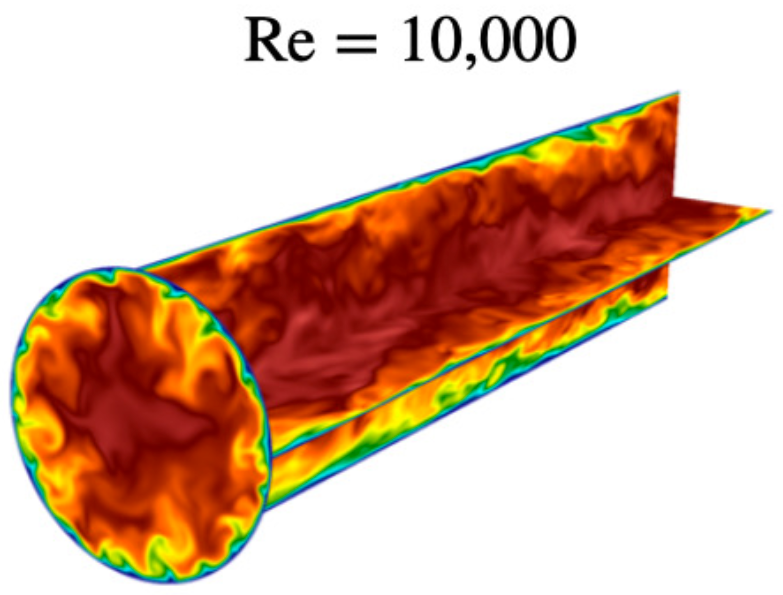
\includegraphics[width = 0.24\textwidth]{figs/kaneko_diss_pipe_r10k.png}}
 \put(1.75,0.00){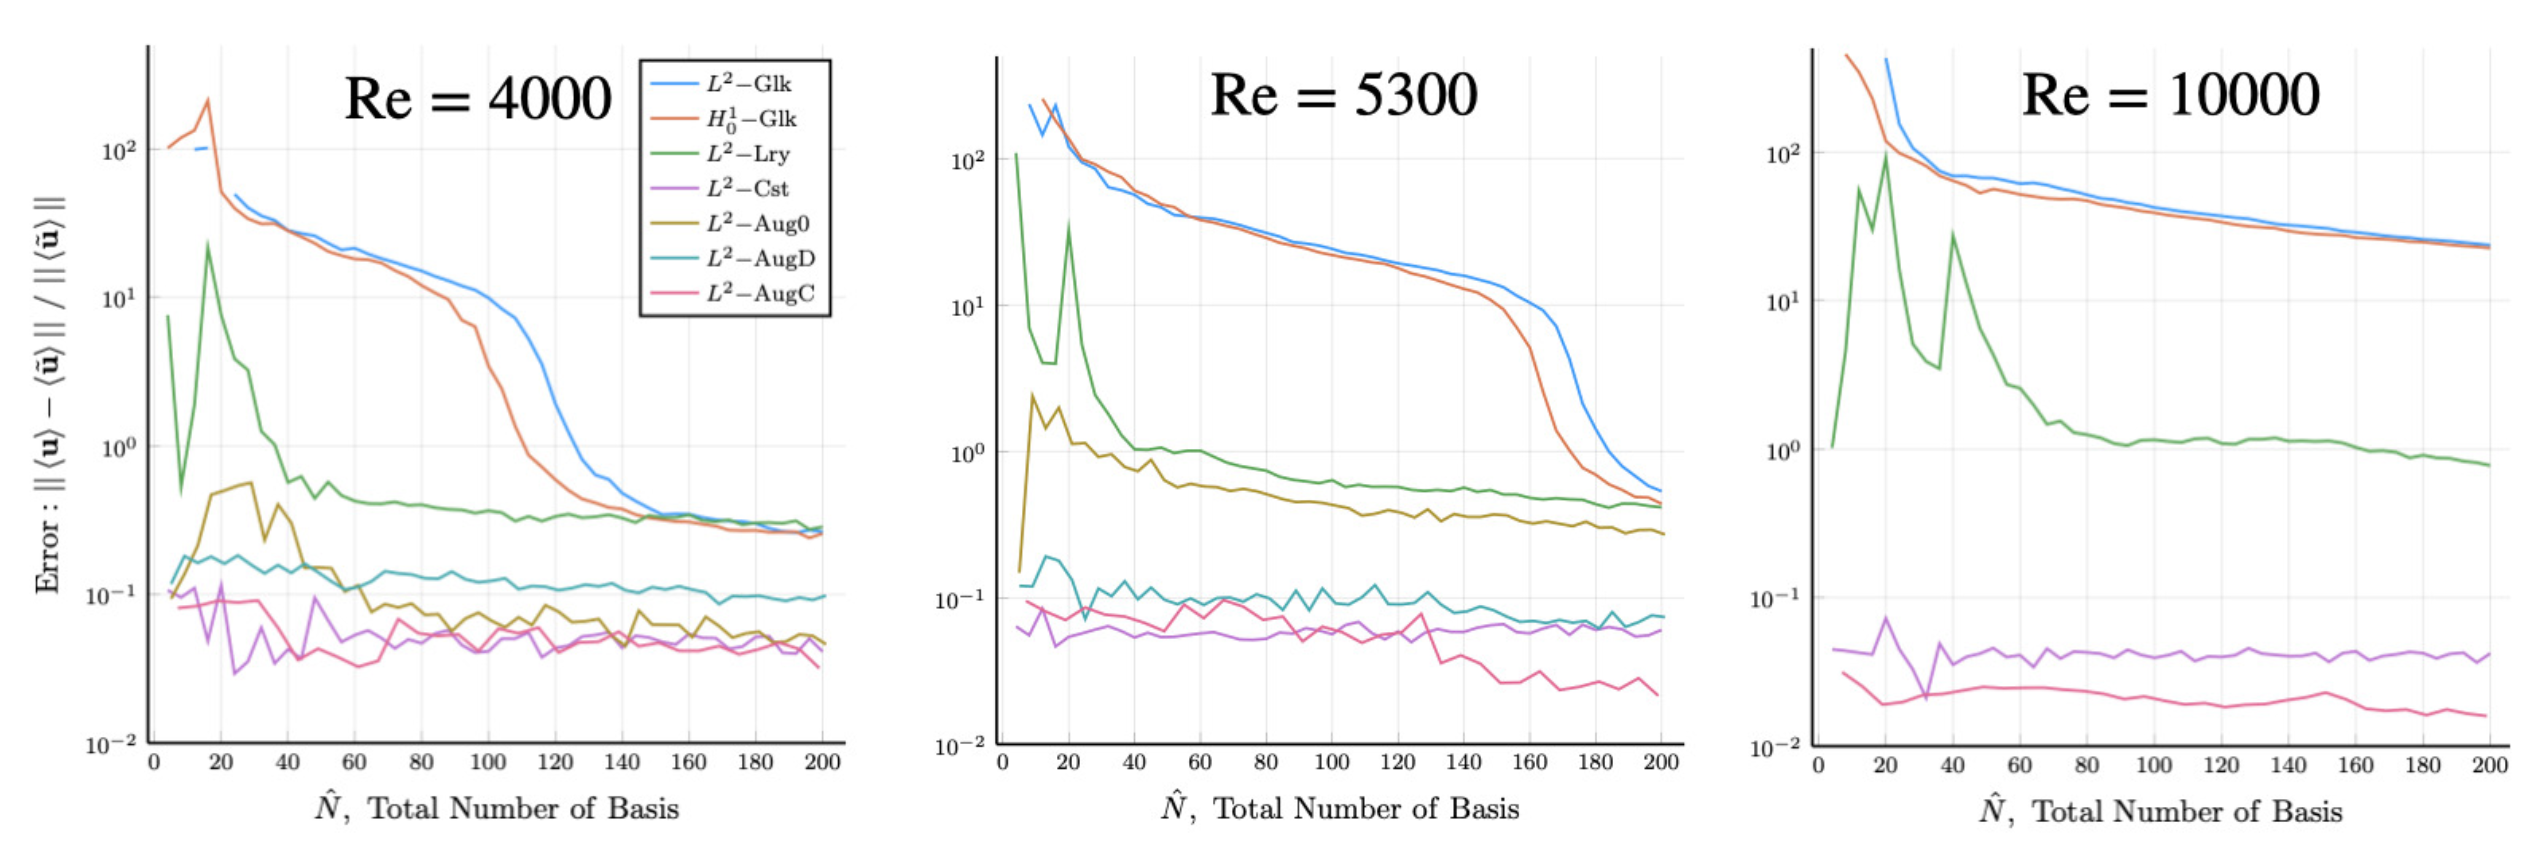
\includegraphics[width = 0.70\textwidth]{figs/kaneko_diss_pipe_ubar.png}}
\end{picture}}
\caption{
\textbf{(left)} Nek5000 DNS of turbulent pipe flow at $Re_D$=10,000;
\textbf{(right)} Mean velocity error in ROM reproduction results for Galerkin POD 
    ($L^2$-Glk, $H^1$-Glk), Leray- and constrainted-based regularization 
    ($L^2$-Lry, $H^1$-Cst), and ABM with three different subsets of the nonlinear terms
    ($L^2$-Aug0=$\bzeta_0 \cdot \nabla \bzeta_j+ \bzeta_j \cdot \nabla \bzeta_0$,
    $L^2$-AugD=$\bzeta_j \cdot \nabla \bzeta_j$,
    $L^2$-AugC=$L^2$-Aug0 $\bigcup$ $L^2$-AugD) \cite{kaneko22a,kaneko22}.
\label{fig:abm}}
\end{figure}

Stability is a requirement for a successful ROM, but it does not guarantee
accuracy of all (or any) of the QOIs.  The standard numerical approach to
improving accuracy is to increase $N$, which can be seen to be beneficial for
the less performant ROMs of Fig. \ref{fig:abm}.  For $Re=4000$, there is a
significant error reduction for the Galerkin ROMs as $N$ is increased from 100
to 140.  For $Re=5300$, the transition occurs for $N=140$ to 180.  For
$N=10,000$, we cannot observe a transition for $N \leq 200$, but one might
speculate that it could be found for sufficiently large $N$.  Unfortunately,
each step of (\ref{eq:erom}) requires a contraction with the 3rd-order tensor
$C_{ijk}$, which requires $O(N^3)$ operations and dominates the cost of the
online (and, potentially, the offline) portion of the ROM.  \textbf{Mitigation of the
$O(N^3)$ cost is of primary importance.}  Possible solutions include replacing
the nonlinear term with an approximation based on the discrete empirical
interpolation method (DEIM) \cite{deim2010} or replacing the rank-3 tensor
$C_{ijk}$ with the sum of $R$ rank-1 tensors, which reduces the $O(N^3)$ cost
to $O(NR)$.  Even if $R=O(N)$, this reduction affords considerable savings, 
implying that one could enrich the approximation space through substantial
increases in $N$.  (An important technical detail is to ensure that the
low-rank tensor inherits the skew-symmetry properties that are intrinsic to
advection operators in closed systems.)

ROMs generally converge faster on small domains, which suggests using
a domain decomposition strategy with (say) $N'=20$ modes on each of $S$
subdomains such that $C_{ijk}$ is sparse with $O(SN'^3)$ nonzeros,
while the number of modes is $N=SN'$.  Such an approach would also
more readily support convective transport of isolated features than
would be possible with an (incomplete) modal basis.  We will investigate
the feasiblity of such an approach for large-domain test cases.


